\chapter{कर्कट जीवविज्ञान}\label{ch:b3:cancer-biology}

इतना बड़ा कोई \omterm{def:b3:cancer-biology:hallmarks}{अर्बुद} कि हाथ से महसूस हो, एक सेंटीमीटर चौड़ा, एक अरब
कोशिकाएँ रखता है और किसी एक बिगड़ी कोशिका से लगभग तीस द्विगुणनों का काम
है --- प्रायः किसी को पता चलने से पहले एक दशक की वृद्धि। उस कोशिका के
पीछे कई उत्परिवर्तन पड़े हैं, जिनमें से हर एक को उसी वंशक्रम में होना
पड़ा और जिनमें से हर एक ने पिछले दो अध्यायों के नियंत्रणों में से एक
हटाया: विभाजन पर कोई ब्रेक, मृत्यु का कोई चालक, विभाजनों की संख्या पर
कोई सीमा, अपनी जगह रहने की कोई शर्त। \omterm{def:b3:cancer-biology:hallmarks}{कर्कट} किसी शरीर के भीतर किसी
कोशिका-समष्टि का उत्परिवर्तन और चयन द्वारा ऐसी अवस्था की ओर विकास है जो
कोशिकाओं के काम आती है और जीव को मार देती है। यह अध्याय उन जीनों को
लेता है जिन पर चोट पड़ती है और जो वे सामान्यतः करते हैं, उस सांख्यिकी
को जो बताती है कि कितने आघात चाहिए, उस शरीरक्रिया को जो किसी \omterm{def:b3:cancer-biology:hallmarks}{अर्बुद} को
एक मिलीमीटर से आगे बढ़ने और फैलने के लिए पानी पड़ती है, उन कारणों को
जिनसे बचा जा सकता है, और उन चिकित्साओं को --- विभाजनशील कोशिकाओं को
मारते विषों से लेकर प्रतिरक्षा-तंत्र को छोड़ देने वाले प्रतिरक्षियों
तक --- जो इस जीवविज्ञान ने संभव की हैं, साथ में उस विकासात्मक कारण के
जिससे वे इतनी बार विफल होती हैं।

\section{कर्कट क्या है}

\begin{definition}[अर्बुद, कर्कट, अभिलक्षण]\label{def:b3:cancer-biology:hallmarks}
\index{कर्कट}\index{अर्बुद}\index{दुर्दम}\index{विक्षेपण}\index{कर्कट के अभिलक्षण}
कोई \emph{अर्बुद} (नववृद्धि) कोशिकाओं का ऐसा क्लोन है जो अपनी वृद्धि के
नियंत्रणों से बच निकला है और किसी ऊतक में जमा होता जाता है। वह
\emph{सौम्य} है यदि वह सीमित और संपुटित रहे, और \emph{दुर्दम} --- कोई
\emph{कर्कट} --- यदि उसकी कोशिकाएँ पड़ोसी ऊतक में घुसें और कहीं और
द्वितीयक अर्बुद बो दें (\emph{विक्षेपण}), और यही मारता है।
कर्कटों के नाम उनकी उद्गम-कोशिका पर हैं: उपकला से कार्सिनोमा
(मानव कर्कटों का \qty{85}{\%}), संयोजी ऊतक से सार्कोमा,
रक्त-निर्माणकारी कोशिकाओं से श्वेतरक्तताएँ और लसीकार्बुद, तंत्रिकाबंध से
ग्लायोमा। ऊतक कोई भी हो, किसी दुर्दम क्लोन ने वही समुच्चय
क्षमताओं का पा लिया होता है, यानी \emph{कर्कट के अभिलक्षण}: वह बिना
किसी बाहरी वृद्धि-संकेत के प्रचुरोद्भवन करता है और उन संकेतों को अनदेखा
करता है जो उसे रोकते; वह \omterm{def:b3:cell-cycle-apoptosis:apoptosis}{एपॉप्टोसिस} का प्रतिरोध करता है; वह
\omterm{def:b3:cancer-biology:telomerase}{टीलोमरेज़} फिर से चालू करके बिना सीमा विभाजित होता है; वह रक्त-वाहिनियाँ
प्रेरित करता है; वह \omterm{def:b3:cancer-biology:metastasis}{घुसपैठ} और विक्षेपण करता है;
और, इन सबके नीचे, उसका जीनोम अस्थिर है, वह ऑक्सीजन में भी अपना उपापचय
ग्लाइकोलयन की ओर पुनःक्रमादेशित करता है (वारबुर्ग प्रभाव), वह ऐसी
शोथकारी कोशिकाएँ बुलाता है जो उसकी मदद करती हैं, और वह प्रतिरक्षा-तंत्र
से बच निकलता है। हर अभिलक्षण सामान्य ऊतक का कोई हारा हुआ नियंत्रण है,
और हर एक जीनों पर उतरता है।
\end{definition}

\begin{omfigure}
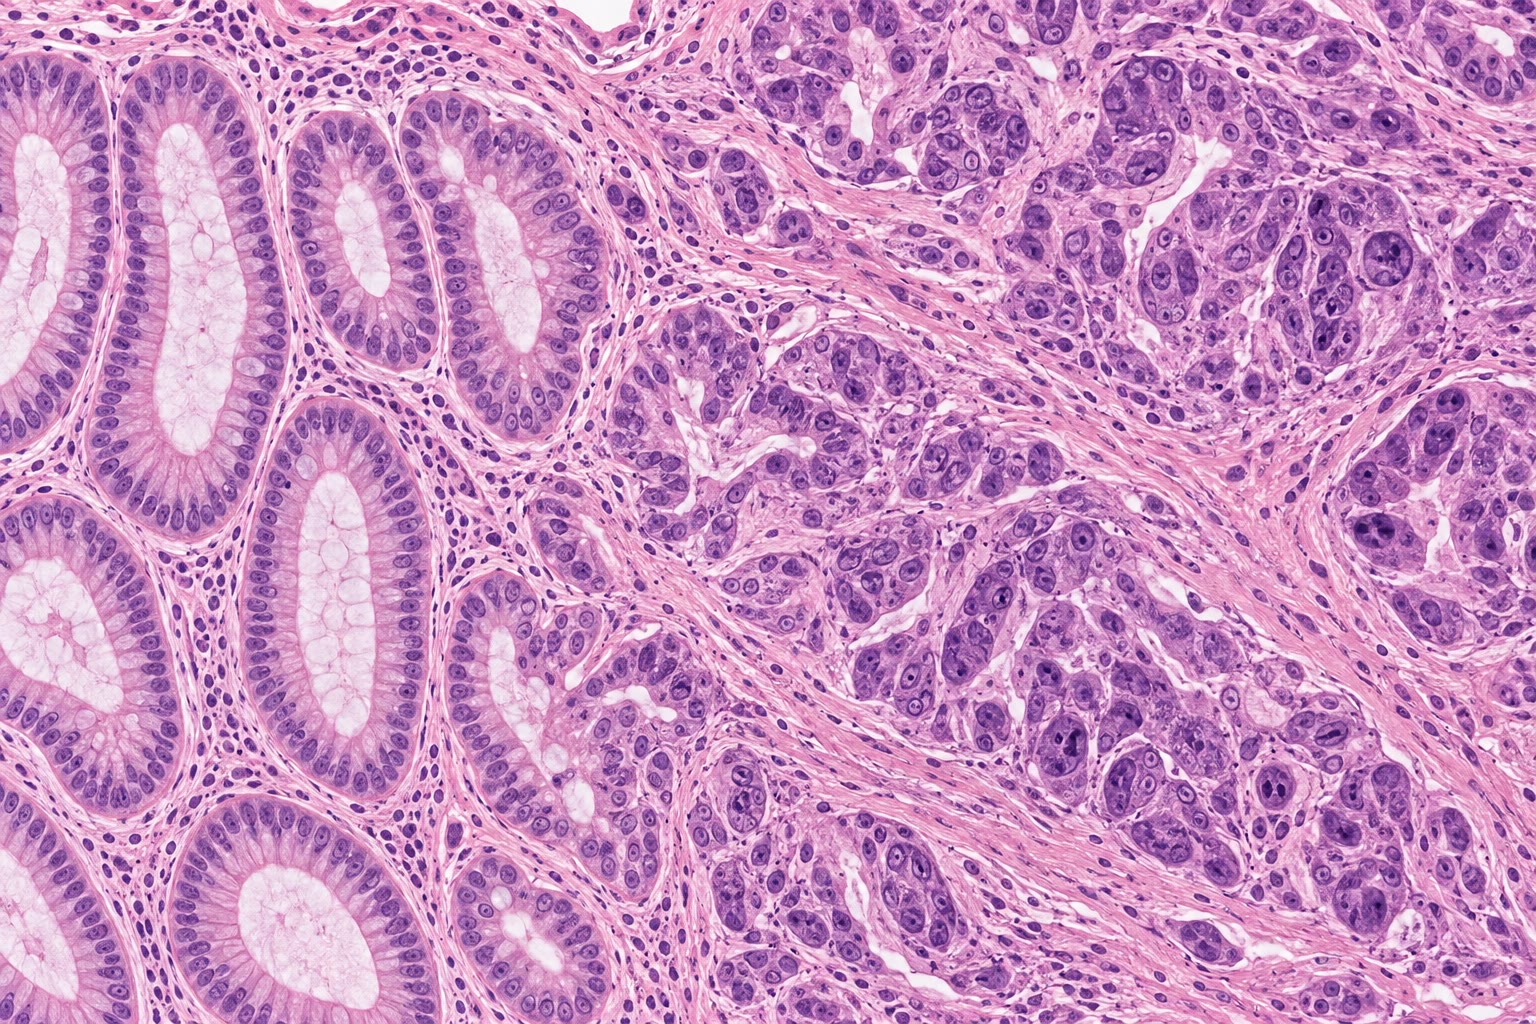
\includegraphics[width=0.56\linewidth]{images/book5/ai/b5-11-tumour-histology.jpg}

{\small अपनी सीमा पर कोई कार्सिनोमा: बाईं ओर नियमित केंद्रकों वाली
सुव्यवस्थित ग्रंथिल उपकला; दाईं ओर बड़े, अनियमित केंद्रकों वाली भीड़ भरी
कोशिकाएँ नीचे के आधारांग में घुसती हुईं --- वही चित्र जिसे कोई
विकृति-विज्ञानी पढ़कर \omterm{def:b3:cancer-biology:hallmarks}{अर्बुद} को \omterm{def:b3:cancer-biology:hallmarks}{दुर्दम} कहता है।}
\end{omfigure}

\section{जिन जीनों पर चोट पड़ती है}

\begin{definition}[कर्कटजीन और अर्बुद-दमनकारी]\label{def:b3:cancer-biology:genes}
\index{कर्कटजीन}\index{आद्य-कर्कट जीन}\index{अर्बुद-दमनकारी जीन}\index{Ras}\index{p53}\index{दो-आघात परिकल्पना}
कोई \emph{आद्य-कर्कट जीन} ऐसा सामान्य जीन है जो प्रचुरोद्भवन या
उत्तरजीविता को बढ़ावा देता है --- कोई वृद्धि कारक, उसका ग्राही, कोई
संकेतन प्रोटीन, कोई अनुलेखन-कारक, कोई \omterm{def:b3:cell-cycle-apoptosis:cdk}{चक्रिन} --- और कोई \emph{कर्कटजीन}
उसका ऐसा उत्परिवर्ती रूप है जो अपने सामान्य संकेत के बिना सक्रिय रहता
है: कोई बिंदु उत्परिवर्तन जो \omterm{def:b3:membrane-traffic:coats}{लघु GTPase} \emph{Ras} को उसकी GTP अवस्था
में बंद कर दे (हर चौथे \omterm{def:b3:cancer-biology:hallmarks}{कर्कट} में ग्लाइसीन~12), ग्राही
HER2 या अनुलेखन-कारक Myc के जीन का प्रवर्धन, कोई स्थानांतरण जो चिरकारी
मज्जाजनी श्वेतरक्तता में \emph{BCR} को काइनेज़ \emph{ABL} से संलयित कर
दे या बर्किट लसीकार्बुद में \emph{MYC} को किसी प्रतिरक्षी संवर्धक के
बगल में रख दे। एक ही उत्परिवर्ती युग्मविकल्पी पर्याप्त है: कर्कटजीन
प्रभावी ढंग से काम करते हैं। कोई \emph{अर्बुद-दमनकारी जीन}
प्रचुरोद्भवन रोकता है या मृत्यु अथवा मरम्मत थोपता है
--- \omterm{def:b3:cell-cycle-apoptosis:checkpoints}{निर्बंधन बिंदु} पर Rb और p16, \emph{p53}, वह रक्षक जो किसी
क्षतिग्रस्त कोशिका को रोक देता या मार देता है, बृहदांत्र के \omterm{prop:b3:cancer-biology:pathways}{Wnt पथ} में
APC, PTEN, BRCA1 और BRCA2, असंगति-मरम्मत जीन --- और योगदान देने के लिए
उसे दोनों युग्मविकल्पी खोने पड़ते हैं: \emph{दो आघात}, जिनमें से पहला
कुलगत \omterm{def:b3:cancer-biology:hallmarks}{कर्कट} संलक्षणों में प्रायः वंशागत होता है और दूसरा कायिक।
\emph{p53} हर दूसरे मानव \omterm{def:b3:cancer-biology:hallmarks}{कर्कट} में उत्परिवर्तित है और शेष में से
अधिकांश में उसका पथ निष्क्रिय।
\end{definition}

\begin{proof}[प्रमाण-सामग्री]
राउस (1911) ने किसी मुर्गी के सार्कोमा को किसी कोशिका-मुक्त छनित से,
यानी किसी विषाणु से, संचरित किया, और उसका एकमात्र रूपांतरणकारी जीन,
\emph{src}, वार्मस तथा बिशप (1976) ने दिखाया कि वह मुर्गी के किसी
सामान्य जीन की पकड़ी गई प्रति है --- \omterm{def:b3:cancer-biology:genes}{कर्कटजीन} बदले हुए कोशिकीय जीन हैं।
वाइनबर्ग (1982) ने किसी मानव मूत्राशय कार्सिनोमा का DNA संवर्धित चूहा-कोशिकाओं
में डाला, जो रूपांतरित हो गईं; ज़िम्मेदार खंड एक ही क्षार के बदलाव वाला
\emph{RAS} था, और वही बदलाव रोगी के सामान्य ऊतक में नहीं था।
नुडसन (1971) ने नेत्र-अर्बुद दृष्टिपटलार्बुद वाले बच्चों की तुलना की:
जिनका कुल-इतिहास था उनमें दोनों आँखों में कई \omterm{def:b3:cancer-biology:hallmarks}{अर्बुद} जल्दी बने; जिनका
नहीं था उनमें एक \omterm{def:b3:cancer-biology:hallmarks}{अर्बुद}, बाद में --- यह इसके अनुरूप है कि कुलगत
स्थितियों को एक कायिक घटना चाहिए और छिटपुट स्थितियों को दो, और इसलिए
ऐसे जीन के अनुरूप जिसकी दोनों प्रतियाँ खोनी पड़ें। \emph{RB}
1986 में क्लोनित हुआ और हर \omterm{def:b3:cancer-biology:hallmarks}{अर्बुद} में सचमुच दोनों युग्मविकल्पी निष्क्रिय
मिले।
\end{proof}

\begin{theorem}[आघात और आयु-वक्र]\label{thm:b3:cancer-biology:armitage-doll}
\index{आर्मिटेज--डॉल प्रतिरूप}\index{बहुचरणी कर्कटजनन}
मान लीजिए किसी \omterm{def:b3:cancer-biology:hallmarks}{कर्कट} को किसी एक कोशिका-वंशक्रम में $k$ स्वतंत्र,
दर-सीमित घटनाएँ चाहिए, जिनमें से हर एक प्रति कोशिका प्रति वर्ष अचर दर
$u$ से होती है, और संवेद्य कोशिकाओं की संख्या $N$ है, $ut \ll 1$ के
साथ। तब इसकी प्रायिकता कि किसी दी हुई कोशिका ने सारी $k$ घटनाएँ
आयु $t$ तक भोग ली हों, लगभग $(ut)^{k}$ है, ऊतक में संचयी जोखिम लगभग
$N(ut)^{k}$ है, और घटना-दर --- आयु $t$ पर प्रति वर्ष नई स्थितियाँ --- है
\[
I(t) \approx N\,k\,u^{k}\,t^{\,k-1},
\]
यानी आयु की कोई घात जिसका घातांक $k - 1$ है: किसी लघुगणक--लघुगणक आलेख पर
$k - 1$ ढाल की एक सरल रेखा। जो व्यक्ति इनमें से एक घटना वंशागत पाता है,
उसके लिए उसी \omterm{def:b3:cancer-biology:hallmarks}{कर्कट} की घटना-दर $\propto t^{\,k-2}$ है, यानी एक घात कम।
\end{theorem}
\begin{proof}
हर घटना, दर $u$ पर, समय $t$ तक प्रायिकता
$1 - e^{-ut} \approx ut$ से हो चुकी होती है; घटनाएँ स्वतंत्र हैं, इसलिए
सारी $k$ प्रायिकता $(ut)^{k}$ से हो चुकी होती हैं, और वे किस क्रम में
हुईं यह यहाँ मायने नहीं रखता। $N$ कोशिकाओं और दुर्लभ घटनाओं के साथ,
जिन कोशिकाओं ने यह अनुक्रम पूरा किया उनकी प्रत्याशित संख्या
$N(ut)^{k}$ है, और घटना-दर उसका काल-अवकलज है, $Nku^{k}t^{k-1}$।
एक घटना वंशागत पाने से $k - 1$ शेष रहती हैं: $(ut)^{k-1}$, घटना-दर
$\propto t^{k-2}$। यदि घटनाओं का क्रम मायने रखता (केवल $1$ क्रम,
$k!$ में से, \omterm{def:b3:cancer-biology:hallmarks}{कर्कट} तक ले जाता) तो पूर्वगुणक बदलता, घातांक नहीं।
\end{proof}

\begin{example}[घातांक पढ़ना]\label{ex:b3:cancer-biology:exponent}
वयस्कों में अधिकांश कार्सिनोमाओं की घटना-दर आयु की लगभग पाँचवीं से
छठी घात से चढ़ती है --- तीस पर प्रति वर्ष लगभग \num{100000} में $1$ से
अस्सी पर $1$ प्रति $300$ तक, यानी $300$ का गुणक आयु के $2.7$ गुने पर, और
$2.7^{5.7} \approx 300$ --- जो छह या सात दर-सीमित घटनाएँ सुझाता है।
यह आकलन मोटा है: हर आघात के बाद किसी क्लोन का फैलाव अगले आघात के जोखिम
वाली कोशिकाओं की संख्या बढ़ा देता है, इसलिए बीच में क्लोनी वृद्धि के
साथ कम घटनाएँ भी वही ढाल दे देती हैं, और अनुक्रमित \omterm{def:b3:cancer-biology:hallmarks}{अर्बुदों} में मिले
\emph{चालक} उत्परिवर्तनों की संख्या दो से आठ है। नुडसन का
दृष्टिपटलार्बुद प्रमेय के दूसरे कथन पर ठीक बैठता है: छिटपुट रोग, जिसे
दो आघात चाहिए, की घटना-दर आयु के साथ चढ़ती है (उन थोड़े वर्षों तक जब
दृष्टिपटलकोरक होते हैं); कुलगत रोग, जिसे एक चाहिए, जन्म से लगभग अचर दर
पर रहता है और जल्दी तथा बार-बार चोट करता है।
\end{example}

\begin{omfigure}
\begin{tikzpicture}
\begin{axis}[
  width=0.68\linewidth, height=6cm,
  xmode=log, ymode=log,
  xmin=20, xmax=100, ymin=1e-6, ymax=1e-1,
  xlabel={आयु (वर्ष)}, ylabel={प्रति व्यक्ति प्रति वर्ष घटना-दर},
  xlabel style={font=\small, at={(axis description cs:0.5,-0.12)}, anchor=north},
  ylabel style={font=\small},
  tick label style={font=\small}, xtick={20,30,50,80}, xticklabels={20,30,50,80},
  clip=false,
]
\addplot[very thick, omThm, domain=20:100, samples=2] {1e-5*(x/30)^5.7};
\addplot[very thick, omDef, domain=20:100, samples=2] {3e-4*(x/30)^1};
\addplot[very thick, omMeth!70!black, domain=20:100, samples=2] {2e-3};
\node[font=\scriptsize, omThm, anchor=south west] at (axis cs:38,2.5e-6) {कार्सिनोमा: ढाल $5$--$6$, छह या सात घटनाएँ};
\node[font=\scriptsize, omDef, anchor=south west] at (axis cs:22,6e-4) {दो आघात: ढाल 1};
\node[font=\scriptsize, omMeth!70!black, anchor=south west] at (axis cs:22,2.3e-3) {एक आघात वंशागत: ढाल 0};
\end{axis}
\end{tikzpicture}

{\small लघुगणकीय अक्षों पर आयु के सामने घटना-दर। जिस \omterm{def:b3:cancer-biology:hallmarks}{कर्कट} को $k$
दर-सीमित घटनाएँ चाहिए वह $t^{k-1}$ की तरह चढ़ता है: वयस्क
कार्सिनोमाओं की तीखी रेखा, और नुडसन की दोनों स्थितियाँ --- कोई
दो-आघात \omterm{def:b3:cancer-biology:hallmarks}{अर्बुद} रैखिक रूप से चढ़ता, और वही \omterm{def:b3:cancer-biology:hallmarks}{अर्बुद} किसी एक वंशागत आघात के
वाहक में, जन्म से अचर दर पर।}
\end{omfigure}

\begin{proposition}[जिन पथों पर चोट पड़ती है]\label{prop:b3:cancer-biology:pathways}
\index{Ras--MAPK पथ}\index{PI3K पथ}\index{Wnt पथ}
सैकड़ों \omterm{def:b3:cancer-biology:hallmarks}{कर्कट} जीन दर्जन भर पथों में आते हैं, और हर \omterm{def:b3:cancer-biology:hallmarks}{अर्बुद} उनमें से किसी
एक को कहीं न कहीं निष्क्रिय कर देता है। वृद्धि-कारक पथ: कोई ग्राही
टायरोसीन काइनेज़ (EGFR, HER2), \omterm{def:b3:cancer-biology:genes}{Ras}, केंद्रक तक जाता काइनेज़-प्रपात
Raf--MEK--ERK, और उसके समांतर उत्तरजीविता तथा वृद्धि की ओर
PI3K--Akt--mTOR, जिसे PTEN रोके रखता है; कोई \omterm{def:b3:cancer-biology:hallmarks}{अर्बुद} उनमें से एक को,
किसी भी जीन के ज़रिए, सक्रिय कर देता है।
\omterm{def:b3:cell-cycle-apoptosis:cdk}{कोशिका-चक्र} का ब्रेक: \omterm{def:b3:cell-cycle-apoptosis:cdk}{चक्रिन} D, Cdk4, p16, Rb (\cref{ch:b3:cell-cycle-apoptosis})।
रक्षक: \omterm{def:b3:cancer-biology:genes}{p53} और उसके नियामक। मृत्यु: Bcl-2। परिवर्धनी
संकेतन: बृहदांत्र में Wnt (APC, $\beta$-कैटेनिन), त्वचा और मस्तिष्क में
हेजहॉग, T~कोशिकाओं में नॉच। जीनोम अनुरक्षण: \omterm{prop:b3:dna-repair:fidelity}{असंगति मरम्मत},
\omterm{def:b3:dna-repair:dsb}{BRCA}, \omterm{def:b3:dna-repair:ddr}{ATM}। \omterm{def:b3:chromatin-epigenetics:nucleosome}{क्रोमैटिन}: \cref{ch:b3:chromatin-epigenetics} के लेखक और
पुनर्रचक, जो हर तीसरे \omterm{def:b3:cancer-biology:hallmarks}{अर्बुद} में उत्परिवर्तित हैं।
अमरता: \omterm{def:b3:cancer-biology:telomerase}{टीलोमरेज़} का प्रवर्तक। चूँकि कोई पथ चरणों की शृंखला है, भिन्न
जीनों के उत्परिवर्तन विकल्प हैं --- उत्परिवर्ती \omterm{def:b3:cancer-biology:genes}{Ras} वाले \omterm{def:b3:cancer-biology:hallmarks}{अर्बुद} में
उत्परिवर्ती EGFR शायद ही साथ मिले --- और किसी एक चरण के विरुद्ध औषधों
को नीचे का कोई उत्परिवर्तन हरा सकता है।
\end{proposition}

\begin{omfigure}
\begin{tikzpicture}[every node/.style={font=\scriptsize}, >=stealth]
  % membrane
  \draw[very thick, omDef] (0,3.6) -- (12,3.6); \draw[very thick, omDef] (0,3.3) -- (12,3.3);
  \node[above] at (1.0,3.65) {बाहर}; \node[below] at (1.0,3.25) {कोशिकाद्रव्य};
  % receptor
  \draw[thick, fill=omProp!35] (3.7,3.0) rectangle (4.1,4.1); \draw[thick, fill=omProp!35] (4.3,3.0) rectangle (4.7,4.1);
  \node[above, align=center] at (4.2,4.15) {वृद्धि कारक $\to$ ग्राही काइनेज़\\(EGFR, HER2)}; \node[right, omThm, font=\tiny] at (4.75,4.0) {प्रवर्धित};
  % Ras
  \node[draw, thick, rounded corners, fill=omDef!20] (ras) at (4.2,2.3) {Ras--GTP};
  \node[right, omThm, font=\tiny] at (5.0,2.3) {G12: सदा चालू};
  \node[draw, thick, rounded corners, fill=omDef!20] (raf) at (4.2,1.4) {Raf $\to$ MEK $\to$ ERK};
  \node[right, omThm, font=\tiny] at (5.8,1.4) {BRAF V600E};
  \node[draw, thick, rounded corners, fill=omMeth!25] (myc) at (4.2,0.4) {Myc, चक्रिन D: प्रचुरोद्भवन};
  \node[right, omThm, font=\tiny] at (6.4,0.4) {Myc प्रवर्धित};
  \draw[->, thick] (4.2,3.0) -- (ras); \draw[->, thick] (ras) -- (raf); \draw[->, thick] (raf) -- (myc);
  % PI3K branch
  \node[draw, thick, rounded corners, fill=omDef!20] (pi3k) at (9.6,2.3) {PI3K $\to$ Akt $\to$ mTOR};
  \node[draw, thick, rounded corners, fill=omMeth!25] (surv) at (9.6,0.4) {उत्तरजीविता, वृद्धि};
  \draw[->, thick] (4.7,3.0) .. controls (6.5,2.8) .. (pi3k.north west); \draw[->, thick] (pi3k) -- (surv);
  \node[draw, thick, rounded corners, fill=omThm!15] (pten) at (12.2,1.4) {PTEN}; \draw[-|, thick, omThm] (pten) -- (9.6,1.4);
  \node[below, omThm, font=\tiny] at (12.2,1.15) {विलोपित};
  % p53 and Rb on the side
  \node[draw, thick, rounded corners, fill=omThm!15] (rb) at (1.2,0.4) {Rb, p16}; \draw[-|, thick, omThm] (rb) -- (myc);
  \node[below, omThm, font=\tiny, align=center] at (1.2,0.15) {दोनों युग्मविकल्पी खोए};
  \node[draw, thick, rounded corners, fill=omThm!15] (p53) at (1.2,1.6) {p53}; \node[below, omThm, font=\tiny, align=center] at (1.2,1.35) {हर दूसरे कर्कट में\\उत्परिवर्तित};
  \draw[-|, thick, omThm] (p53) -- (1.2,0.65);
\end{tikzpicture}

{\small वृद्धि-कारक पथ और \omterm{def:b3:cancer-biology:hallmarks}{कर्कट} उन पर कहाँ चोट करते हैं। हरे डिब्बे
निर्गत हैं, नीले वे संकेतन-चरण जिन्हें कर्कटजनक उत्परिवर्तन चालू बंद
कर देते हैं, लाल वे दमनकारी जिन्हें \omterm{def:b3:cancer-biology:hallmarks}{अर्बुद} खो देते हैं (पट्टियाँ
निरोध चिह्नित करती हैं)। कोई \omterm{def:b3:cancer-biology:hallmarks}{अर्बुद} प्रायः इस आरेख में एक सक्रियकारी और
एक-दो निष्क्रियकारी घाव ढोता है।}
\end{omfigure}

\section{कोई अर्बुद विकसित होता है}

\begin{proposition}[बहुचरणी कर्कटजनन]\label{prop:b3:cancer-biology:multistep}
\index{चालक उत्परिवर्तन}\index{यात्री उत्परिवर्तन}\index{क्लोनी विकास}\index{उत्परिवर्तनी हस्ताक्षर}
कोई \omterm{def:b3:cancer-biology:hallmarks}{अर्बुद} कायिक विकास का उत्पाद है: उत्परिवर्तन विचरण पैदा करता है, और
ऊतक के भीतर चयन उन्हीं को वरीयता देता है जो अधिक विभाजित हों, कम मरें
या किसी बंधन से बच निकलें। फ़ोगेलश्टाइन द्वारा सुलझाया गया
बृहदांत्रीय अनुक्रम आदर्श है: \emph{APC} का ह्रास कोई छोटा सौम्य
अंकुर बनाता है; कोई \emph{KRAS} उत्परिवर्तन उसे किसी ग्रंथ्यर्बुद तक
बढ़ने देता है; \emph{SMAD4} या \emph{TP53} का ह्रास उसे कार्सिनोमा में
बदल देता है; आगे के बदलाव \omterm{def:b3:cancer-biology:metastasis}{घुसपैठ} की छूट देते हैं। हर चरण कोई क्लोनी
फैलाव है जो अगले के जोखिम वाली कोशिकाएँ गुणा कर देता है। कोई अनुक्रमित
\omterm{def:b3:cancer-biology:hallmarks}{अर्बुद} हज़ारों उत्परिवर्तन ढोता है, जिनमें से मुट्ठी भर --- प्रायः दो
से आठ --- ऐसे \emph{चालक} हैं जिन्होंने वरणीय लाभ दिया; बाकी
\emph{यात्री} हैं, जो क्लोन में साथ ढोए गए, और उनका वर्णक्रम इसका लेखा
है कि उन्हें किसने बनाया: मेलानोमा में पराबैंगनी प्रकाश से सटे
पिरिमिडीनों पर C$\to$T, फेफड़े के \omterm{def:b3:cancer-biology:hallmarks}{कर्कट} में तंबाकू के धुएँ से
G$\to$T, APOBEC एंज़ाइमों के, दोषपूर्ण \omterm{prop:b3:dna-repair:fidelity}{असंगति मरम्मत} के और ऐफ़्लाटॉक्सिन
के अँगुलि-चिह्न --- यानी \emph{\omterm{prop:b3:cancer-biology:multistep}{उत्परिवर्तनी हस्ताक्षर}}। \omterm{def:b3:cancer-biology:hallmarks}{अर्बुद} विषम
होते हैं, उपक्लोनों का एक शाखित वृक्ष, और जो उपक्लोन मारता है वह निदान
के समय प्रायः अल्पसंख्यक होता है।
\end{proposition}

\begin{omfigure}
\begin{tikzpicture}[every node/.style={font=\scriptsize}, >=stealth]
  \foreach \x/\lab/\gene/\col/\r in {0/{सामान्य उपकला}/{}/omDef!20/0.5, 2.6/{छोटा अंकुर}/{APC खोया (दोनों युग्मविकल्पी)}/omDef!35/0.7, 5.4/{ग्रंथ्यर्बुद}/{KRAS सक्रिय}/omProp!40/1.0, 8.4/{कार्सिनोमा}/{SMAD4 या TP53 खोया}/omThm!35/1.3, 11.6/{घुसपैठी, विक्षेपित}/{और चालक,\\अस्थिरता}/omThm!60/1.5} {
    \draw[thick, fill=\col] (\x,0) circle (\r);
    \node[below, align=center] at (\x,-1.6) {\lab};
    \node[above, align=center, omThm] at (\x,1.6) {\gene};
  }
  \foreach \a/\b in {0.5/1.9, 3.3/4.4, 6.4/7.1, 9.7/10.1} \draw[->, very thick] (\a,0) -- (\b,0);
  \node[below] at (5.8,-2.3) {दस से तीस वर्ष; हर चरण कोई क्लोनी फैलाव जो अगले के जोखिम वाली कोशिकाएँ गुणा कर देता है};
\end{tikzpicture}

{\small बृहदांत्रीय अनुक्रम। हर \omterm{prop:b3:cancer-biology:multistep}{चालक उत्परिवर्तन} किसी क्लोन को फैलाता
है, और फैला हुआ क्लोन वे कोशिकाएँ देता है जिनमें अगला चालक उठ सकता है;
पूरा रास्ता दशकों लेता है, इसीलिए अंकुरों की जाँच \omterm{def:b3:cancer-biology:hallmarks}{कर्कट} रोक देती है।}
\end{omfigure}

\begin{method}[एम्स परीक्षण]\label{met:b3:cancer-biology:ames}
\index{एम्स परीक्षण}\index{उत्परिवर्तजन}
यह जाँचने के लिए कि कोई रसायन उत्परिवर्तजनक है या नहीं, और इसलिए
संभावित कर्कटजन है या नहीं: (1) \emph{Salmonella} की ऐसी प्रजाति लीजिए
जिसमें किसी हिस्टिडीन-जैवसंश्लेषी जीन में कोई बिंदु उत्परिवर्तन हो और
जो हिस्टिडीन के बिना उग न सके; (2) रसायन को किसी यकृत-निष्कर्ष से
मिलाइए, जिसके एंज़ाइम अनेक यौगिकों को उनके सक्रिय उत्परिवर्तजनक रूपों
में बदल देते हैं, जैसे शरीर करता; (3) कोई $10^{8}$ जीवाणु उस मिश्रण के
साथ हिस्टिडीन-रहित ऐगार पर फैलाइए;
(4) जो बस्तियाँ उगें उन्हें गिनिए --- हर एक कोई ऐसी प्रत्यावर्ती है
जिसमें किसी नए उत्परिवर्तन ने जीन बहाल कर दिया; (5) स्वतःस्फूर्त दर से
तुलना कीजिए। प्रत्यावर्तियों में मात्रा-निर्भर वृद्धि का अर्थ है कि
यौगिक बिंदु उत्परिवर्तन करता है। अधिकांश ज्ञात कर्कटजन धनात्मक आते
हैं; परीक्षण सस्ता है, दो दिन लेता है, और जो यौगिक उसमें विफल हो उसकी
और जाँच बनाए जाने से पहले होती है।
\end{method}

\begin{definition}[अमरता और अस्थिरता]\label{def:b3:cancer-biology:telomerase}
\index{टीलोमरेज़}\index{गुणसूत्री अस्थिरता}\index{असुगुणिता!कर्कट में}
सामान्य कायिक कोशिकाओं में टीलोमरेज़ नहीं होती और वे अपने विभाजन
टीलोमियर की लंबाई में गिनती हैं (\cref{ch:b3:stem-cells}): कोई पचास के
बाद वे जराग्रस्त हो जाती हैं, और जो कोशिका \omterm{def:b3:cancer-biology:genes}{p53} तथा Rb खोकर \omterm{def:b3:cell-cycle-apoptosis:other}{जरावस्था}
लाँघ जाए वह तब तक चलती है जब तक उसके टीलोमियर चुक न जाएँ और उसके
गुणसूत्र जुड़कर टूटने न लगें --- कोई संकट जो अधिकांश क्लोन मार देता है।
जो विरला बच जाता है उसने \emph{टीलोमरेज़} फिर चालू कर ली होती है,
प्रायः किसी प्रवर्तक उत्परिवर्तन से, और वह अमर है; \qty{90}{\%} \omterm{def:b3:cancer-biology:hallmarks}{कर्कट}
वह एंज़ाइम अभिव्यक्त करते हैं। संकट अपने निशान छोड़ जाता है: जुड़े और
टूटे गुणसूत्र, प्रवर्धन, विलोपन, स्थानांतरण --- यानी
\emph{गुणसूत्री अस्थिरता}, जो तर्कु जाँच-बिंदु के ह्रास और गलत बँटवारे
पर \omterm{def:b3:cancer-biology:genes}{p53} की अनुक्रिया के ह्रास के साथ मिलकर अधिकांश ठोस \omterm{def:b3:cancer-biology:hallmarks}{अर्बुदों} को
असुगुणित बना देती है और उन्हें लगातार विचरण पैदा करते रहने देती है।
इसके बजाय थोड़े-से \omterm{def:b3:cancer-biology:hallmarks}{अर्बुदों} में \omterm{prop:b3:dna-repair:fidelity}{असंगति मरम्मत} खो जाने से कोई
उत्परिवर्तक लक्षण-प्ररूप होता है, जिसमें गुणसूत्र-प्ररूप सामान्य रहता
है और बिंदु-उत्परिवर्तन दर हज़ार गुना।
\end{definition}

\section{ऊतक के रूप में अर्बुद}

\begin{proposition}[ऑक्सीजन बिना वाहिनी के अर्बुद का आकार तय करती है]\label{prop:b3:cancer-biology:oxygen}
\index{रक्तवाहिनीजनन}\index{विसरण सीमा}\index{अल्पऑक्सीयता}
ऐसे ऊतक पर विचार कीजिए जो प्रति इकाई आयतन अचर दर $q$ से ऑक्सीजन खपाता
है और जिसे किसी वाहिनी से विसरण (गुणांक $D$) द्वारा आपूर्ति होती है,
जिसकी दीवार पर सांद्रता $c_{0}$ है। स्थायी अवस्था पर एक विमा में $D\,
\mathrm{d}^{2}c/\mathrm{d}x^{2} = q$ होता है, इसलिए
$c(x) = c_{0} - qx^{2}/2D$ और ऑक्सीजन इस दूरी पर चुक जाती है
\[
L = \sqrt{\frac{2Dc_{0}}{q}} .
\]
$D = \qty{2e-9}{m^2/s}$, $c_{0} = \qty{0.05}{mol/m^3}$ और $q =
\qty{0.03}{mol/m^3/s}$ (कोई श्वसन करता \omterm{def:b3:cancer-biology:hallmarks}{अर्बुद}) के साथ $L \approx \qty{80}{\micro
m}$: कोई भी कोशिका किसी केशिका से लगभग सौ माइक्रोमीटर से अधिक दूर जीवित
नहीं रह सकती। इसलिए जिस क्लोन की अपनी कोई वाहिनी न हो वह एक से दो
मिलीमीटर के व्यास पर रुक जाता है, जिसका केंद्र परिगलित और किनारा
जीवित रहता है। आगे बढ़ने के लिए उसे \emph{रक्तवाहिनीजनन} प्रेरित करना
पड़ता है --- उसकी अल्पऑक्सी कोशिकाएँ अनुलेखन-कारक HIF को स्थिर करती हैं,
जो VEGF प्रेरित करता है, जो पास की अंतःकलीय कोशिकाओं को उसकी ओर अंकुरित
करता है। जूडा फ़ोकमैन ने 1971 में प्रस्ताव किया कि इस चरण को रोकने से
\omterm{def:b3:cancer-biology:hallmarks}{अर्बुद} भूखे मर जाएँगे; VEGF के विरुद्ध प्रतिरक्षी अब कई \omterm{def:b3:cancer-biology:hallmarks}{कर्कटों} में
मानक हैं, यद्यपि \omterm{def:b3:cancer-biology:hallmarks}{अर्बुद} उनके अनुकूल हो जाते हैं।
\end{proposition}
\begin{proof}
स्थायी अवस्था पर विसरणी अभिवाह $-D\,\mathrm{d}c/\mathrm{d}x$ को
$x$ के साथ ठीक उतनी ही तेज़ी से बदलना चाहिए जितनी तेज़ी से ऑक्सीजन
खपती है: $\mathrm{d}(-D\,
\mathrm{d}c/\mathrm{d}x)/\mathrm{d}x = -q$, यानी $D c'' = q$।
$c(0) = c_{0}$ और उस गहराई पर $c'(L) = 0$ के साथ, जहाँ कुछ बचा ही न हो
(उसके आगे कोई अभिवाह नहीं), दो बार समाकलन करने पर $c = c_{0} - qx^{2}/2D$
मिलता है, और $c(L) = 0$ काम में आता है $L$ तय करने के लिए। संख्याएँ
इसके बाद निकलती हैं।
\end{proof}

\begin{omfigure}
\begin{tikzpicture}
\begin{axis}[
  width=0.6\linewidth, height=5.4cm,
  axis x line=bottom, axis y line=left,
  xmin=0, xmax=120, ymin=0, ymax=0.06,
  xlabel={केशिका से दूरी ($\unit{\micro m}$)}, ylabel={ऑक्सीजन ($\unit{mol/m^3}$)},
  xlabel style={font=\small, at={(axis description cs:0.5,-0.12)}, anchor=north},
  ylabel style={font=\small},
  tick label style={font=\small}, xtick={0,40,80,120}, ytick={0,0.025,0.05},
  clip=false,
]
\addplot[very thick, omDef, domain=0:81.6, samples=40] {0.05 - 0.03*(x*1e-6)^2/(2*2e-9)};
\addplot[very thick, omDef, domain=81.6:120, samples=2] {0};
\fill[omThm!25] (axis cs:81.6,0) rectangle (axis cs:120,0.06);
\node[font=\scriptsize, omThm!70!black, anchor=south, align=center] at (axis cs:100,0.03) {ऑक्सीजन नहीं:\\परिगलन};
\node[font=\scriptsize, omDef, anchor=south west] at (axis cs:5,0.052) {$c(x) = c_{0} - qx^{2}/2D$};
\draw[dashed, gray] (axis cs:81.6,0) -- (axis cs:81.6,0.06); \node[font=\scriptsize, anchor=south west] at (axis cs:83,0.002) {$L$};
\end{axis}
\end{tikzpicture}

{\small श्वसन करते ऊतक में ऑक्सीजन निकटतम केशिका से दूरी के साथ किसी
परवलय की तरह गिरती है और $L = \sqrt{2Dc_{0}/q}$ पर चुक जाती है, जो यहाँ
लगभग \qty{80}{\micro m} है। बिना वाहिनियों के कोई \omterm{def:b3:cancer-biology:hallmarks}{अर्बुद} किसी मृत
क्रोड के चारों ओर उतनी ही मोटाई का जीवित कोशिकाओं का खोल है।}
\end{omfigure}

\begin{omfigure}
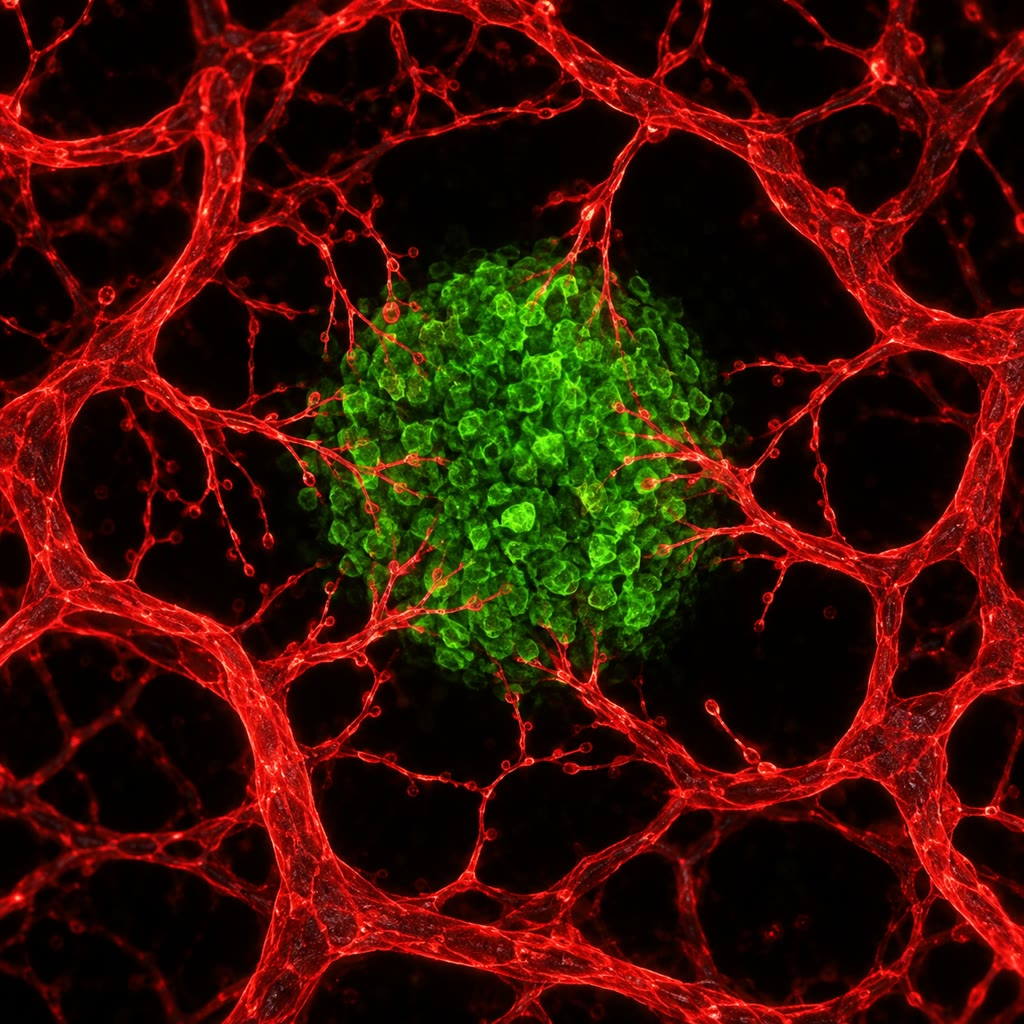
\includegraphics[width=0.36\linewidth]{images/book5/ai/b5-11-angiogenesis.jpg}\hspace{0.04\linewidth}
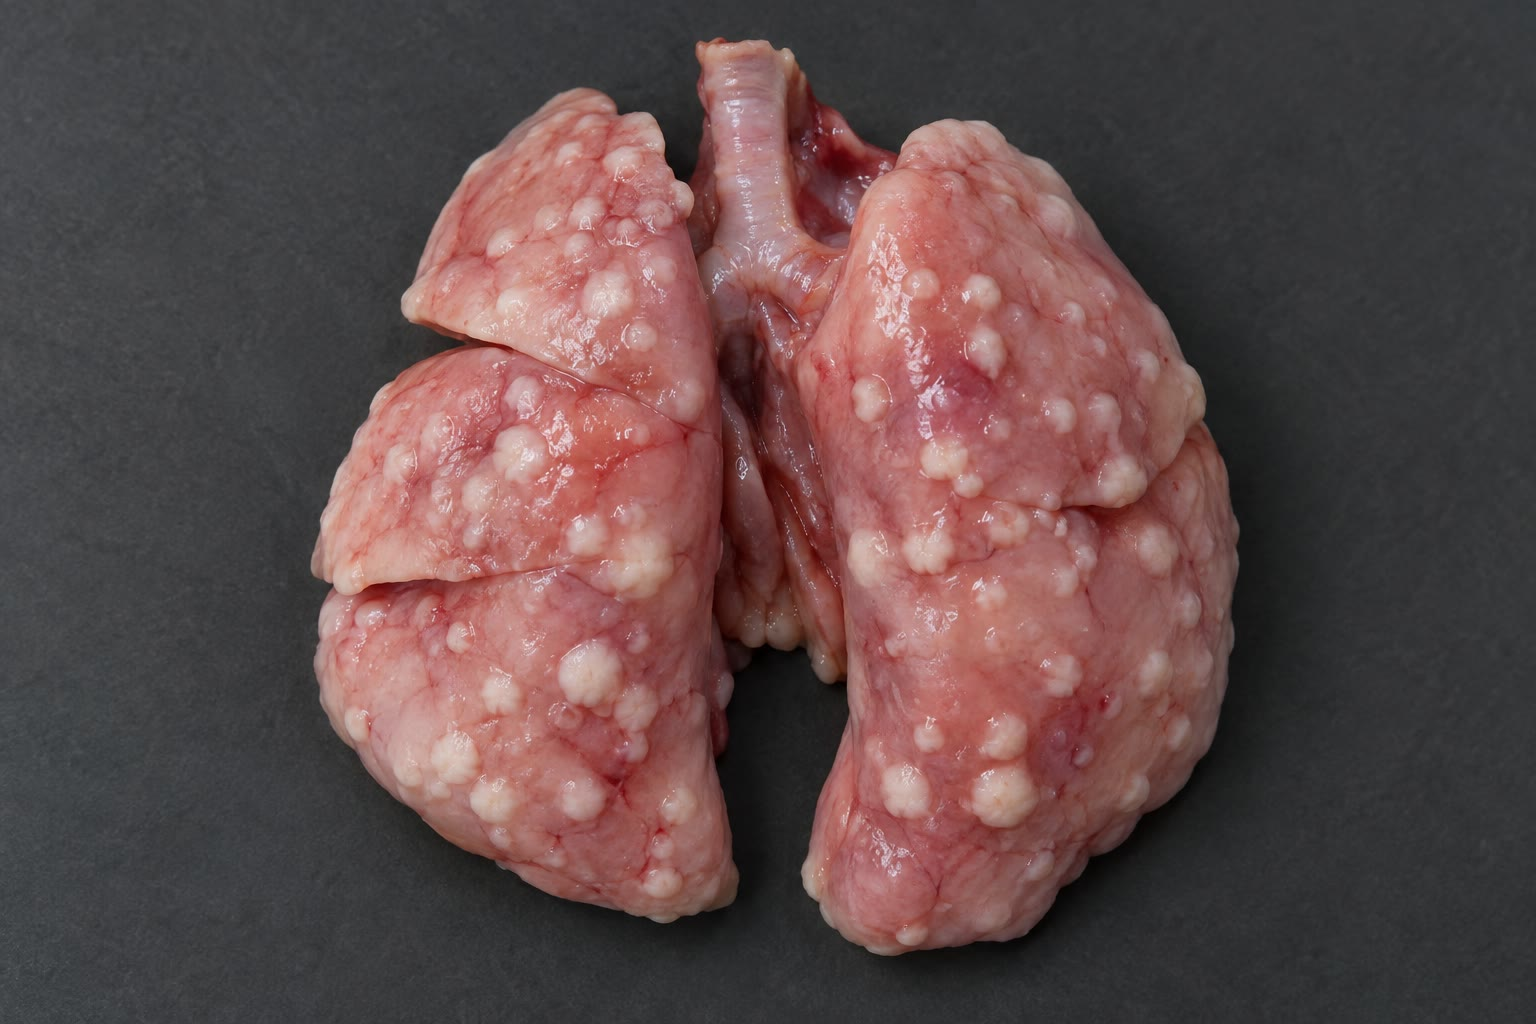
\includegraphics[width=0.54\linewidth]{images/book5/ai/b5-11-metastasis-lung.jpg}

{\small बाएँ: कोई अर्बुद-गोलिका (हरी) किसी पड़ोसी जाल से नई वाहिनियाँ
(लाल) बुलाती हुई --- संवर्धन में रक्तवाहिनीजनन। दाएँ: विक्षेपों से जड़ा
किसी चूहे का फेफड़ा, जिसका हर उपनिवेश किसी एक कोशिका ने बसाया जो रक्त
की यात्रा से बच निकली।}
\end{omfigure}

\begin{definition}[घुसपैठ और विक्षेपण]\label{def:b3:cancer-biology:metastasis}
\index{घुसपैठ}\index{उपकला--मध्यजनोतकी संक्रमण}\index{बीज और मिट्टी}
\omterm{def:b3:cancer-biology:hallmarks}{विक्षेपण} के लिए किसी कार्सिनोमा कोशिका को उपकला छोड़नी पड़ती है ---
अपनी कोशिका-संधियाँ और ध्रुवता खोकर गतिशीलता पानी पड़ती है, यानी कोई
\emph{उपकला--मध्यजनोतकी संक्रमण} जिसे वे अनुलेखन-कारक चलाते हैं जो
सामान्यतः भ्रूणीय परिवर्धन में काम आते हैं --- स्रावित प्रोटिएज़ों से
आधार-झिल्ली और आधात्री का अपघटन करना पड़ता है, किसी रक्त या लसीका
वाहिनी की दीवार पार करनी पड़ती है, परिसंचरण में बचना पड़ता है (दस हज़ार
में एक से भी कम बचती है, क्योंकि उन्हें अपरूपण, जुड़ाव का अभाव और
प्राकृतिक घातक कोशिकाएँ मार देती हैं), किसी दूसरे अंग की केशिका-शय्या
में अटकना पड़ता है, बाहर निकलना पड़ता है, और वहाँ बढ़ना पड़ता है। वह
कहाँ बढ़ती है यह यादृच्छिक नहीं: स्तन-कर्कट हड्डी, फेफड़े, यकृत और
मस्तिष्क जाता है, बृहदांत्र-कर्कट यकृत को, पौरुष-ग्रंथि \omterm{def:b3:cancer-biology:hallmarks}{कर्कट} हड्डी को
--- 1889 का पेजेट का \emph{बीज और मिट्टी}, जिसकी व्याख्या कुछ
रक्त-प्रवाह से और कुछ कोशिका तथा ऊतक के संकेतों के मेल से होती है। कोई
प्रकीर्ण कोशिका बढ़ने से पहले वर्षों तक सुप्त पड़ी रह सकती है,
इसीलिए \omterm{def:b3:cancer-biology:hallmarks}{कर्कट} स्पष्ट इलाज के एक दशक बाद लौट आते हैं। ठोस \omterm{def:b3:cancer-biology:hallmarks}{अर्बुदों} से
होने वाली दस में नौ मृत्युएँ \omterm{def:b3:cancer-biology:hallmarks}{विक्षेपण} से होती हैं, और यही वह चरण है जो
सबसे कम समझा गया है।
\end{definition}

\begin{proposition}[प्रतिरक्षा-तंत्र से बचना]\label{prop:b3:cancer-biology:immune}
\index{प्रतिरक्षा-अपवंचन}\index{जाँच-बिंदु निरोधक}\index{नवप्रतिजन}
किसी \omterm{def:b3:cancer-biology:hallmarks}{अर्बुद} के उत्परिवर्तन \emph{नवप्रतिजन} बनाते हैं, यानी ऐसे
पेप्टाइड जो कोई सामान्य कोशिका प्रस्तुत नहीं करती, और कोशिकाविषी
T~कोशिकाएँ \omterm{def:b3:cancer-biology:hallmarks}{अर्बुद} कोशिकाओं को पहचानकर मार देती हैं --- यही कारण है कि
प्रतिरक्षा-दमित रोगियों में अधिक \omterm{def:b3:cancer-biology:hallmarks}{कर्कट} होते हैं और यही कि अनेक
उत्परिवर्तनों वाले \omterm{def:b3:cancer-biology:hallmarks}{अर्बुद} (मेलानोमा, फेफड़ा, असंगति-मरम्मत-अपर्याप्त
बृहदांत्र) प्रतिरक्षा-चिकित्सा पर सबसे अच्छी अनुक्रिया देते हैं। कोई
चिकित्सकीय रूप से स्पष्ट \omterm{def:b3:cancer-biology:hallmarks}{अर्बुद} वही है जो बच निकला है: उन MHC अणुओं को
खोकर जो पेप्टाइड प्रस्तुत करते हैं, दमनकारी कारक स्रावित करके, नियामक
T~कोशिकाएँ बुलाकर, और सबसे बढ़कर PD-L1 अभिव्यक्त करके, जो T~कोशिकाओं
पर निरोधी ग्राही PD-1 से जुड़कर उन्हें बंद कर देता है --- वही ब्रेक जो
सामान्यतः किसी प्रतिरक्षा-अनुक्रिया को समाप्त करता है
(\cref{ch:b3:adaptive-immunity})। जो प्रतिरक्षी PD-1 या PD-L1 को, या
पहले वाले ब्रेक CTLA-4 को, रोकते हैं वे T~कोशिकाएँ छोड़ देते हैं; रोगियों
के एक अंश में --- \omterm{def:b3:cancer-biology:hallmarks}{अर्बुद} के अनुसार पाँचवें से आधे तक --- वे उन \omterm{def:b3:cancer-biology:hallmarks}{कर्कटों}
की टिकाऊ उपशांति करते हैं जो अनुपचार्य थे, और उनके दुष्प्रभाव
स्व-प्रतिरक्षा हैं, यानी उसी ब्रेक का दूसरा काम।
\end{proposition}

\section{कारण और उपचार}

\begin{proposition}[कारण]\label{prop:b3:cancer-biology:causes}
\index{कर्कटजन}\index{कर्कटजनक विषाणु}
\omterm{def:b3:cancer-biology:hallmarks}{कर्कट} वह सब पैदा करता है जो प्रमेय की घटनाओं की दर या जोखिम वाली
कोशिकाओं की संख्या बढ़ा दे। \emph{रासायनिक कर्कटजन}, जिनमें से अधिकांश
यकृत द्वारा सक्रिय किए जाने के बाद उत्परिवर्तजन हैं: तंबाकू के धुएँ के
सत्तर कर्कटजन, जो एक-तिहाई कर्कट-मृत्युएँ करते हैं और फेफड़े के \omterm{def:b3:cancer-biology:hallmarks}{कर्कट}
का जोखिम पंद्रह से पच्चीस गुना बढ़ा देते हैं; फफूँदी लगे अनाज का
ऐफ़्लाटॉक्सिन; ऐस्बेस्टस, जो उत्परिवर्तजन नहीं बल्कि कोई जीर्ण उत्तेजक
है। \emph{विकिरण}: त्वचा के लिए पराबैंगनी प्रकाश
(\cref{ch:b3:dna-repair} के द्विलक), श्वेतरक्तता, अवटु
और स्तन के लिए आयनकारी विकिरण। \emph{संक्रमण}, यानी संसार भर के छठे
हिस्से \omterm{def:b3:cancer-biology:hallmarks}{कर्कट}: पैपिलोमा विषाणु, जिनके प्रोटीन E6 और E7 \omterm{def:b3:cancer-biology:genes}{p53} नष्ट करते और
Rb निष्क्रिय करते हैं और लगभग सारे ग्रीवा-कर्कट करते हैं (अब कोई टीका
उन्हें रोक देता है); यकृत-कर्कट में हेपटाइटिस B और C विषाणु;
लसीकार्बुदों में एप्स्टाइन--बार विषाणु; आमाशय-कर्कट में
\emph{Helicobacter pylori}, दशकों के शोथ के ज़रिए। कुछ \qty{5}{\%}
\omterm{def:b3:cancer-biology:hallmarks}{कर्कटों} में किसी अर्बुद-दमनकारी में \emph{वंशागत उत्परिवर्तन}, यानी
जन्म पर ही पहला आघात। और संयोग: किसी \omterm{def:b3:cancer-biology:hallmarks}{अर्बुद} के अधिकांश उत्परिवर्तन
प्रतिकृति की साधारण त्रुटियों से उठे, इसलिए जो ऊतक सबसे अधिक विभाजित
होते हैं --- बृहदांत्र, त्वचा, रक्त --- उनमें सबसे अधिक \omterm{def:b3:cancer-biology:hallmarks}{कर्कट} होते हैं,
और जोखिम आयु के साथ चढ़ता है, कोई कुछ भी करे।
\end{proposition}

\begin{theorem}[एक औषध क्यों विफल होती है और दो शायद नहीं]\label{thm:b3:cancer-biology:goldie-coldman}
\index{गोल्डी--कोल्डमैन प्रतिरूप}\index{औषध प्रतिरोध}\index{संयोजन चिकित्सा}
मान लीजिए $N$ कोशिकाओं का कोई \omterm{def:b3:cancer-biology:hallmarks}{अर्बुद} एक ही कोशिका से क्रमिक विभाजनों
द्वारा बना है, और किसी दी हुई औषध के प्रति प्रतिरोध देने वाला कोई
उत्परिवर्तन प्रति कोशिका-विभाजन दर $\mu$ से उठता है। तब इसकी प्रायिकता
कि उपचार शुरू होते समय \omterm{def:b3:cancer-biology:hallmarks}{अर्बुद} में \emph{कोई} प्रतिरोधी कोशिका न हो,
लगभग यह है
\[
P_{0} \approx e^{-\mu N},
\]
इसलिए $\mu N \gg 1$ के लिए प्रतिरोध लगभग निश्चित रूप से पहले से मौजूद
रहता है। स्वतंत्र प्रतिरोध-क्रियाविधियों वाली दो औषधों के लिए, दोनों के
प्रति प्रतिरोधी कोई कोशिका प्रति विभाजन लगभग दर $\mu_{1}\mu_{2}$ से
उठती है, और $P_{0}
\approx e^{-\mu_{1}\mu_{2}N}$: $N = 10^{9}$ और $\mu = 10^{-7}$ के साथ,
एक औषध औसतन $\mu N = 100$ प्रतिरोधी क्लोनों का सामना करती है, और दो
औषधें इस बात की प्रायिकता $10^{-5}$ कि कोई एक भी दोहरा-प्रतिरोधी कोशिका
हो।
\end{theorem}
\begin{proof}[आंशिक प्रमाण]
$1$ से $N$ कोशिकाओं तक बढ़ने में कुल लगभग $N$ विभाजन लगते हैं ($N$
पत्तों वाले किसी वृक्ष में $N - 1$ आंतरिक शीर्ष होते हैं)। यदि हर विभाजन
पर प्रायिकता $\mu$ से कोई प्रतिरोधी कोशिका बने और, पहले सन्निकटन में,
उसके वंशज न मरें न बाकी से आगे बढ़ें, तो प्रतिरोध-घटनाओं की संख्या माध्य
$\mu N$ के साथ पॉइसों है, और एक भी न होने की प्रायिकता $e^{-\mu N}$ है।
स्वतंत्र क्रियाविधियाँ प्रति-विभाजन प्रायिकताओं का गुणन करती हैं।
यह सन्निकटन इस बात की उपेक्षा करता है कि अगेते उत्परिवर्ती बड़े
प्रतिरोधी क्लोन छोड़ते हैं --- पूरा बंटन लूरिया और डेलब्रुक का है,
जिसे वर्ष~2 के खंड में लिया गया है --- पर \emph{किसी भी} उत्परिवर्ती के
न होने की प्रायिकता, जो यह तय करती है कि \omterm{def:b3:cancer-biology:hallmarks}{अर्बुद} ठीक हो सकता है या नहीं,
ठीक वही पॉइसों पद है।
\end{proof}

\begin{example}[चिकित्साएँ और उनका तर्क]\label{ex:b3:cancer-biology:therapy}
शल्य और विकिरण-चिकित्सा किसी स्थानिक \omterm{def:b3:cancer-biology:hallmarks}{अर्बुद} को हटाते या मारते हैं;
विकिरण \omterm{def:b3:dna-repair:lesions}{द्विलड़ी विखंडनों} से मारता है, और उसे दैनिक मात्राओं में बाँटने
से सामान्य ऊतक बीच में मरम्मत कर लेता है (\cref{ch:b3:dna-repair})।
कोशिकाविषी रसायन-चिकित्सा --- क्षारकारी कारक, प्रति-उपापचयज,
सूक्ष्मनलिका-विष, सांस्थितिकी-एंज़ाइम निरोधक --- किसी भी प्रकार की
विभाजनशील कोशिकाएँ मारती है, \omterm{def:b3:cancer-biology:hallmarks}{अर्बुद} कोशिकाएँ कुछ अधिक, और
\emph{लघुगणकीय-वध} नियम का पालन करती है: हर बारी एक अचर अंश मारती है,
मान लीजिए \qty{99}{\%}, जिससे छह बारियाँ $10^{12}$ कोशिकाएँ घटाकर एक कर
देती हैं, और \omterm{def:b3:cancer-biology:hallmarks}{अर्बुद} बड़ा हो या छोटा, वही छह बारियाँ चाहिए;
रोगी के बाल, आँत और मज्जा, जो विभाजित होते हैं, मात्रा तय करते हैं।
लक्षित चिकित्सा उस घाव पर वार करती है जिस पर \omterm{def:b3:cancer-biology:hallmarks}{अर्बुद} निर्भर है: इमैटिनिब
BCR--ABL काइनेज़ रोकती है और उसने चिरकारी मज्जाजनी श्वेतरक्तता को घातक
रोग से चिरकारी रोग बना दिया; ट्रैस्टुज़ुमैब HER2 से बँधता है; पिछले
अध्यायों के PARP निरोधक, Cdk4/6 निरोधक और वेनेटोक्लैक्स हर एक किसी एक
दोष का लाभ उठाते हैं। प्रतिरक्षा-चिकित्सा T~कोशिकाएँ छोड़ देती है। और
प्रमेय बताती है कि उन्हें कैसे काम में लेना चाहिए: संयोजन में, जल्दी,
जब $N$ सबसे छोटा हो --- शल्य के बाद सहायक रसायन-चिकित्सा यही करती है
--- और ऐसी औषधों से जिनकी प्रतिरोध-क्रियाविधियाँ न मिलती हों।
\omterm{def:b3:cancer-biology:hallmarks}{अर्बुद} कोई विकसित होती समष्टि है, और उपचार ही चयन है।
\end{example}

\begin{omfigure}
\begin{tikzpicture}
\begin{axis}[
  width=0.7\linewidth, height=5.6cm,
  axis x line=bottom, axis y line=left,
  xmin=0, xmax=8, ymin=1, ymax=1e13, ymode=log,
  xlabel={रसायन-चिकित्सा की बारियाँ}, ylabel={अर्बुद कोशिकाएँ},
  xlabel style={font=\small, at={(axis description cs:0.5,-0.12)}, anchor=north},
  ylabel style={font=\small},
  tick label style={font=\small}, xtick={0,2,4,6,8},
  clip=false,
]
\addplot[very thick, omDef, mark=*, mark size=1.2pt] coordinates {(0,1e12) (1,1e10) (2,1e8) (3,1e6) (4,1e4) (5,1e2) (6,1)};
\addplot[very thick, omThm, mark=*, mark size=1.2pt] coordinates {(0,1e12) (1,1.01e10) (2,1.02e8) (3,1.04e6) (4,1.1e4) (5,200) (6,300) (7,600) (8,1200)};
\addplot[dashed, gray, domain=0:8, samples=2] {1e9};
\node[font=\scriptsize, gray, anchor=south west] at (axis cs:0.2,1.3e9) {पकड़ में आने योग्य, $10^{9}$};
\node[font=\scriptsize, omDef, anchor=south west] at (axis cs:0.3,1e4) {प्रति बारी \qty{99}{\%} वध};
\node[font=\scriptsize, omThm, anchor=south west] at (axis cs:5.2,3e3) {आरंभ में एक प्रतिरोधी कोशिका: पुनरावर्तन};
\end{axis}
\end{tikzpicture}

{\small लघुगणकीय-वध नियम। हर बारी कोशिकाओं का वही अंश मारती है, इसलिए
\omterm{def:b3:cancer-biology:hallmarks}{अर्बुद} प्रति बारी एक नियत संख्या में दशमलव-कोटियाँ सिकुड़ता है और समाप्त
होने से बहुत पहले पकड़ से बाहर हो जाता है (नीला); पहले से मौजूद कोई एक
प्रतिरोधी कोशिका हर बारी बच जाती है और फिर बढ़ जाती है (लाल)।}
\end{omfigure}

\begin{remark}[क्या बदला है]\label{rem:b3:cancer-biology:changed}
किसी धनी देश में \omterm{def:b3:cancer-biology:hallmarks}{कर्कट} का निदान पाने वाले आधे रोगी अब दस वर्ष जीते हैं,
1970 के एक-चौथाई के सामने। यह लाभ रोकथाम से आया (तंबाकू, हेपटाइटिस और
पैपिलोमा विषाणु के टीके, अंकुरों तथा ग्रीवा-घावों की जाँच), जल्दी पकड़
से, और इस अध्याय के जीवविज्ञान से निकले उपचारों से --- वह संयोजन
रसायन-चिकित्सा जो अधिकांश बाल-श्वेतरक्तताएँ और वृषण-कर्कट ठीक कर देती
है, लक्षित औषधें, और प्रतिरक्षा-चिकित्साएँ। जो नहीं बदला वह विक्षेपित
रोग है, जिसे जीवविज्ञान समझा तो देता है पर अभी ठीक नहीं करता; अगले लाभ
\omterm{def:b3:cancer-biology:hallmarks}{अर्बुद} को वही मानकर आएँगे जो वह है, यानी उपचार द्वारा थोपे गए चयन के
अंतर्गत विकसित होती एक समष्टि।
\end{remark}

\section{अभ्यास}

\begin{exercise}[$\star$]\label{exo:b3:cancer-biology:1}
किसी \omterm{def:b3:cancer-biology:genes}{कर्कटजीन} को किसी \omterm{def:b3:cancer-biology:genes}{अर्बुद-दमनकारी जीन} से क्रियाविधि में, बदलने वाले
युग्मविकल्पियों की संख्या में, और हर एक के दो उदाहरणों सहित अलग कीजिए।
\end{exercise}

\begin{exercise}[$\star$]\label{exo:b3:cancer-biology:2}
\omterm{def:b3:cancer-biology:hallmarks}{कर्कट के अभिलक्षण} गिनाइए और हर एक के लिए इस या किसी पिछले अध्याय के ऐसे
एक जीन का नाम दीजिए जिसका बदलाव उसे देता है।
\end{exercise}

\begin{exercise}[$\star$]\label{exo:b3:cancer-biology:3}
नुडसन ने कुलगत और छिटपुट दृष्टिपटलार्बुद के बारे में क्या देखा, और
उन्होंने क्या निष्कर्ष निकाला?
\end{exercise}

\begin{exercise}[$\star$]\label{exo:b3:cancer-biology:4}
\omterm{met:b3:cancer-biology:ames}{एम्स परीक्षण} समझाइए और यह भी कि यकृत-निष्कर्ष क्यों जोड़ा जाता है।
\end{exercise}

\begin{exercise}[$\star\star$]\label{exo:b3:cancer-biology:5}
किसी \omterm{def:b3:cancer-biology:hallmarks}{कर्कट} की घटना-दर प्रति वर्ष $2\times 10^{-5}$ है, आयु $40$ पर,
और $2\times 10^{-3}$, आयु $80$ पर। आयु-घात नियम का घातांक और उससे
सुझाई गई दर-सीमित घटनाओं की संख्या आँकिए।
\end{exercise}

\begin{exercise}[$\star\star$]\label{exo:b3:cancer-biology:6}
$D =
\qty{2e-9}{m^2/s}$ और $c_{0} = \qty{0.05}{mol/m^3}$ के साथ
\cref{prop:b3:cancer-biology:oxygen} का उपयोग करते हुए
\qty{0.01}{mol/m^3/s} खपाते ऊतक के लिए और उससे तीन गुना खपाते किसी
\omterm{def:b3:cancer-biology:hallmarks}{अर्बुद} के लिए $L$ निकालिए। तेज़ी से बढ़ता \omterm{def:b3:cancer-biology:hallmarks}{अर्बुद} जल्दी परिगलित क्यों हो
जाता है?
\end{exercise}

\begin{exercise}[$\star\star$]\label{exo:b3:cancer-biology:7}
$10^{11}$ कोशिकाओं के किसी \omterm{def:b3:cancer-biology:hallmarks}{अर्बुद} का उपचार ऐसी औषध से होता है जो प्रति
बारी \qty{99.9}{\%} मारती है। उसे एक कोशिका से नीचे लाने में कितनी
बारियाँ लगेंगी? दो बारियों के बाद \omterm{def:b3:cancer-biology:hallmarks}{अर्बुद} पकड़ में क्यों नहीं आता जबकि
$10^{5}$ कोशिकाएँ बची हैं, और उपचार रोकने के लिए इसका क्या अर्थ है?
\end{exercise}

\begin{exercise}[$\star\star$]\label{exo:b3:cancer-biology:8}
समझाइए कि EGFR का कोई उत्परिवर्तन और KRAS का कोई उत्परिवर्तन एक ही
फेफड़ा-अर्बुद में शायद ही क्यों मिलते हैं, और किसी EGFR निरोधक से
उपचारित \omterm{def:b3:cancer-biology:hallmarks}{अर्बुद} प्रायः KRAS उत्परिवर्तन के साथ क्यों लौट आता है।
\end{exercise}

\begin{exercise}[$\star\star$]\label{exo:b3:cancer-biology:9}
पैपिलोमा विषाणु के प्रोटीन E6 और E7 \omterm{def:b3:cancer-biology:genes}{p53} तथा Rb को निष्क्रिय करते हैं।
समझाइए कि इससे ग्रीवा-कर्कट कैसे चलता है, उसमें दशक क्यों लगते हैं, और
लैंगिक क्रिया से पहले दिया गया कोई टीका उसे क्यों रोक देता है।
\end{exercise}

\begin{exercise}[$\star\star\star$]\label{exo:b3:cancer-biology:10}
आर्मिटेज--डॉल तर्क का विस्तार कीजिए ताकि हर आघात अगले से पहले अपने
क्लोन को गुणक $g$ से फैला सके: दिखाइए कि घटना-दर में $t$ की वही घात
रहती है पर पूर्वगुणक $g^{k-1}$ से गुणा हो जाता है, और चर्चा कीजिए कि
किसी आयु-वक्र से निकाला गया $k$ चालकों की संख्या की ऊपरी सीमा क्यों है।
\end{exercise}

\begin{exercise}[$\star\star\star$]\label{exo:b3:cancer-biology:11}
\cref{thm:b3:cancer-biology:goldie-coldman} के साथ तुलना कीजिए कि (क)
$10^{9}$-कोशिका \omterm{def:b3:cancer-biology:hallmarks}{अर्बुद} का उपचार छह बारी औषध A से और फिर छह बारी औषध B
से किया जाए, और (ख) A तथा B आरंभ से साथ दी जाएँ, जब $\mu_{A} =
\mu_{B} = 10^{-7}$ हो। हर रणनीति के लिए $P_{0}$ निकालिए और समझाइए कि
अगेता संयोजन नियम क्यों है।
\end{exercise}

\begin{exercise}[$\star\star\star$]\label{exo:b3:cancer-biology:12}
पीटो का विरोधाभास: किसी हाथी में किसी मनुष्य से सौ गुना कोशिकाएँ हैं
और वह उतना ही जीता है, फिर भी उसे अधिक \omterm{def:b3:cancer-biology:hallmarks}{कर्कट} नहीं होता। इस अध्याय की
प्रमेय से बताइए कि भोली अपेक्षा क्या है, और दो ऐसी क्रियाविधियाँ
सुझाइए जिनसे बड़े प्राणी यह समस्या हल कर सकते थे (हाथी में
\emph{TP53} की बीस प्रतियाँ हैं)।
\end{exercise}

\section{समस्या: किसी अर्बुद का अंकगणित}

\begin{problem}[{सप्तांत समस्या --- एक कोशिका से उगाया और पकड़ में आने
तक समयबद्ध किया गया कोई अर्बुद, आघातों की संख्या के लिए उसका आयु-वक्र
पढ़ा गया, उसकी ऑक्सीजन-आपूर्ति तथा परिगलित क्रोड निकाले गए, और उसका
उपचार प्रतिरोध की निश्चितता के सामने नियोजित किया गया, जिसका अंत पकड़
में आने तक के वर्षों, किसी वाहिनी के चारों ओर जीवित अर्बुद की गहराई और
इस प्रायिकता पर होता है कि कोई संयोजन ठीक कर देगा}]
\label{pb:b3:cancer-biology:1}
आँकड़े: किसी \omterm{def:b3:cancer-biology:hallmarks}{अर्बुद} कोशिका का आयतन \qty{1000}{\micro m^3}; द्विगुणन-काल
\qty{100}{d}; पकड़ \qty{1}{cm^3} पर; घातक भार \qty{1}{kg}।
आयु-वक्र: घटना-दर प्रति वर्ष $1\times 10^{-5}$, $30$ पर, और $3\times
10^{-3}$, $80$ पर। ऑक्सीजन: $D = \qty{2e-9}{m^2/s}$, $c_{0} =
\qty{0.05}{mol/m^3}$, \omterm{def:b3:cancer-biology:hallmarks}{अर्बुद} में $q = \qty{0.03}{mol/m^3/s}$; किसी
वाहिनीयुक्त \omterm{def:b3:cancer-biology:hallmarks}{अर्बुद} में केशिकाएँ \qty{150}{\micro m} की दूरी पर हैं।
चिकित्सा: हर बारी \qty{99}{\%} मारती है; प्रति औषध प्रति विभाजन
प्रतिरोध-उत्परिवर्तन दर $10^{-7}$; हर तीन सप्ताह में एक बारी; \omterm{def:b3:cancer-biology:hallmarks}{अर्बुद}
बारियों के बीच उसी द्विगुणन-काल से फिर बढ़ता है।

\medskip
\noindent\textbf{भाग I --- वृद्धि।}
\begin{enumerate}
  \item \qty{1}{cm^3} में कितनी कोशिकाएँ? एक कोशिका से कितने
        द्विगुणन?
  \item संस्थापक कोशिका से पकड़ तक कितने वर्ष?
  \item पकड़ से घातक भार तक कितने द्विगुणन, और कितने वर्ष? दोनों
        अंतरालों की तुलना कीजिए।
  \item अनेक \omterm{def:b3:cancer-biology:hallmarks}{अर्बुद} \qty{1}{cm^3} पर पकड़ में आते हैं पर केवल पाँच
        वर्ष से बढ़ रहे थे। आरंभ में द्विगुणन-काल के बारे में, या
        वृद्धि-नियम के बारे में, क्या सच रहा होगा?
  \item किसी \omterm{def:b3:cancer-biology:hallmarks}{अर्बुद} में किसी भी समय केवल कोशिकाओं का कोई अंश $f$
        विभाजित होता है (वृद्धि-अंश), और कोई अंश मरता है। यदि कोशिकाएँ
        \qty{2}{d} में चक्र लगाएँ पर \omterm{def:b3:cancer-biology:hallmarks}{अर्बुद} $100$ में दोगुना हो, तो
        इससे जन्म और मृत्यु के संतुलन के बारे में क्या निकलता है?
  \item वही लघुगणकीय-वध रसायन-चिकित्सा किसी धीरे बढ़ते \omterm{def:b3:cancer-biology:hallmarks}{अर्बुद} को किसी
        तेज़ \omterm{def:b3:cancer-biology:hallmarks}{अर्बुद} से अधिक क्यों छोड़ देती है, और फिर भी तेज़ वाला
        बारियों के बीच अधिक तेज़ी से क्यों बढ़ जाता है?
\end{enumerate}

\medskip
\noindent\textbf{भाग II --- आघात।}
\begin{enumerate}[resume]
  \item दोनों घटना-दरों से आयु-वक्र का घातांक $k - 1$ और उससे निहित
        घटनाओं की संख्या $k$ निकालिए।
  \item यदि हर घटना प्रति कोशिका प्रति वर्ष $u = 10^{-6}$ से हो,
        $N = 10^{8}$ संवेद्य कोशिकाओं में, तो प्रमेय आयु $70$ तक संचयी
        जोखिम का क्या पूर्वानुमान करती है, आपके $k$ के साथ? क्या वह
        प्रशंसनीय है? क्या छूट रहा है?
  \item गुणक $g = 100$ से क्लोनी फैलाव मानकर, पहले $k - 1$ आघातों में
        से हर एक के बाद,
        \cref{exo:b3:cancer-biology:10} का उपयोग करते हुए दोहराइए।
  \item कोई वाहक एक आघात वंशागत पाती है। यदि बाकी दरें अपरिवर्तित हों
        तो आयु $40$ पर उसकी घटना-दर किस गुणक से बढ़ जाती है?
        ($(ut)^{k-1}$ की तुलना $(ut)^{k}$ से कीजिए, $t = 40$ पर।)
  \item धूम्रपान इनमें से एक घटना के लिए $u$ को $10$ गुना कर देता है।
        यदि वह घटना $k$ में से एक हो तो घटना-दर किस गुणक से चढ़ती है;
        और यदि वह उनमें से दो हो तो?
  \item समझाइए कि पचास पर धूम्रपान छोड़ना फेफड़े के \omterm{def:b3:cancer-biology:hallmarks}{कर्कट} का जोखिम किसी
        चालू धूम्रपायी से नीचे क्यों ले आता है, पर कभी किसी कभी न
        धूम्रपान करने वाले जितना नहीं।
\end{enumerate}

\medskip
\noindent\textbf{भाग III --- आपूर्ति।}
\begin{enumerate}[resume]
  \item \omterm{def:b3:cancer-biology:hallmarks}{अर्बुद} में ऑक्सीजन की प्रवेश-गहराई $L$ निकालिए।
  \item बिना वाहिनी की कोई गोलिका: वह अधिकतम व्यास क्या है जिस पर हर
        कोशिका को ऑक्सीजन मिले? \qty{2}{mm} की किसी गोलिका के जीवित
        किनारे की मोटाई क्या है, और उसके आयतन का कितना अंश जीवित है?
  \item \qty{150}{\micro m} की दूरी पर केशिकाओं वाले किसी वाहिनीयुक्त
        \omterm{def:b3:cancer-biology:hallmarks}{अर्बुद} में क्या हर कोशिका को ऑक्सीजन मिलती है? कौन-सी कोशिकाएँ
        अल्पऑक्सी हैं, और यह विकिरण-चिकित्सा के लिए (ऑक्सीजन विकिरण की
        क्षति को पक्का कर देती है) और p53-उत्परिवर्ती कोशिकाओं के चयन
        के लिए क्यों मायने रखता है?
  \item कोई औषध \omterm{def:b3:cancer-biology:hallmarks}{अर्बुद} की केशिका-सघनता आधी कर देती है। दूरी फिर से
        निकालिए और बताइए कि वाहिनियों के बीचोबीच की कोशिकाओं का क्या
        होता है।
  \item अल्पऑक्सी कोशिकाएँ ग्लाइकोलयन पर चली जाती हैं और प्रति
        ग्लूकोज़ $30$ के बजाय \qty{2}{ATP} बनाती हैं। अपनी ATP आपूर्ति
        बनाए रखने के लिए उन्हें ग्लूकोज़-ग्रहण किस गुणक से बढ़ाना पड़ता
        है, और \omterm{def:b3:cancer-biology:hallmarks}{अर्बुदों} के चित्रण में इसका उपयोग कैसे होता है?
  \item समझाइए कि अकेली प्रति-रक्तवाहिनीजनन चिकित्सा शायद ही क्यों ठीक
        करती है पर रसायन-चिकित्सा को \omterm{def:b3:cancer-biology:hallmarks}{अर्बुद} तक पहुँचने में मदद कर सकती है।
\end{enumerate}

\medskip
\noindent\textbf{भाग IV --- उपचार।}
\begin{enumerate}[resume]
  \item \qty{1}{cm^3} के किसी \omterm{def:b3:cancer-biology:hallmarks}{अर्बुद} का उपचार एक औषध से होता है।
        पुनर्वृद्धि और प्रतिरोध की उपेक्षा करते हुए कितनी बारियाँ उसे
        एक कोशिका से नीचे ले आती हैं?
  \item बारियों के बीच (तीन सप्ताह) बचे हुए फिर बढ़ते हैं। किस गुणक
        से? प्रति चक्र शुद्ध वध और आवश्यक चक्रों की संख्या फिर से
        निकालिए।
  \item उपचार के आरंभ पर औषध के प्रति प्रतिरोधी कोशिकाओं की प्रत्याशित
        संख्या और इसकी प्रायिकता निकालिए कि कोई भी न हो।
  \item स्वतंत्र क्रियाविधियों वाली दो औषधें साथ दी जाती हैं। आरंभ पर
        कोई दोहरा-प्रतिरोधी कोशिका न होने की प्रायिकता?
        $10^{12}$ कोशिकाओं के \omterm{def:b3:cancer-biology:hallmarks}{अर्बुद} पर?
  \item सहायक चिकित्सा शल्य के बाद दी जाती है, जब शायद $10^{6}$
        कोशिकाएँ अनपकड़ी रह जाती हैं। एक और दो औषधों के लिए
        प्रायिकताएँ फिर से निकालिए, और पाठ बताइए।
  \item कोई प्रतिरक्षा-चिकित्सा ऐसी T~कोशिकाएँ प्रेरित करती है जो
        किसी भी नवप्रतिजन प्रस्तुत करती कोशिका को मार देती हैं। उसके
        प्रति प्रतिरोध किसी काइनेज़ निरोधक के प्रति प्रतिरोध से भिन्न
        समस्या क्यों है, और प्रमेय के अनुसार वह किन \omterm{def:b3:cancer-biology:hallmarks}{अर्बुदों} पर सबसे
        अच्छा काम करना चाहिए?
  \item सारांश दीजिए: संस्थापक कोशिका से पकड़ तक के वर्ष
        (प्रश्न~2), किसी वाहिनी के चारों ओर जीवित \omterm{def:b3:cancer-biology:hallmarks}{अर्बुद} की गहराई
        (प्रश्न~13), और इसकी प्रायिकता कि \qty{1}{cm^3} के किसी
        \omterm{def:b3:cancer-biology:hallmarks}{अर्बुद} में दो-औषध संयोजन को कोई प्रतिरोधी कोशिका न मिले
        (प्रश्न~22)।
\end{enumerate}
\end{problem}
